\chapter{Tasks and schedule}
\label{chap:tasks}

The main tasks involving this project are:
\begin{enumerate}
    \item Deliver the \emph{Requirement Analysis and Specification Document}, containing the goals, the domain assumptions, and the functional and nonfunctional requirements of the software syste.
    \item Deliver the \emph{Design Document}, containing the architecture and the design of the software system.
    \item Deliver the \emph{Integration Testing Plan Document}, containing the strategy to perform integration testing on the system.
    \item Deliver the \emph{Project Plan}, which is this document.
    \item Prepare a brief presentation (\~15 min) of the delivered documents to our client, using slides.
    \item Develop the software system and write unit tests.
    \item Perform integration testing on the system.
\end{enumerate}

Please note that, as new requirements can emerge, new choices are made and the development proceeds, all these tasks can be iterated before the conclusion of the development. In particular, unit and integration testing will be continuously performed throughout the development process. The dependency graph for the tasks is shown in~\autoref{fig:tasks-dag}.

The first five tasks for the project are already defined by the document about the project rules~\cite{se-project-rules}, together with the deadlines for the delivery of the RASD, the Design Document and the ITPD.
So, those activities are already scheduled.

There are no fixed deadlines, instead, for the development of the software. From the COCOMO estimation, we expect the development to last X months, so it will be presumably finished by MM 2016.
% TODO insert dates based on COCOMO estimation

The schedule for our project is outlined in~\autoref{tab:schedule}. The Gantt chart for the project is shown in~\autoref{fig:gantt}.

\begin{figure}
    \centering
    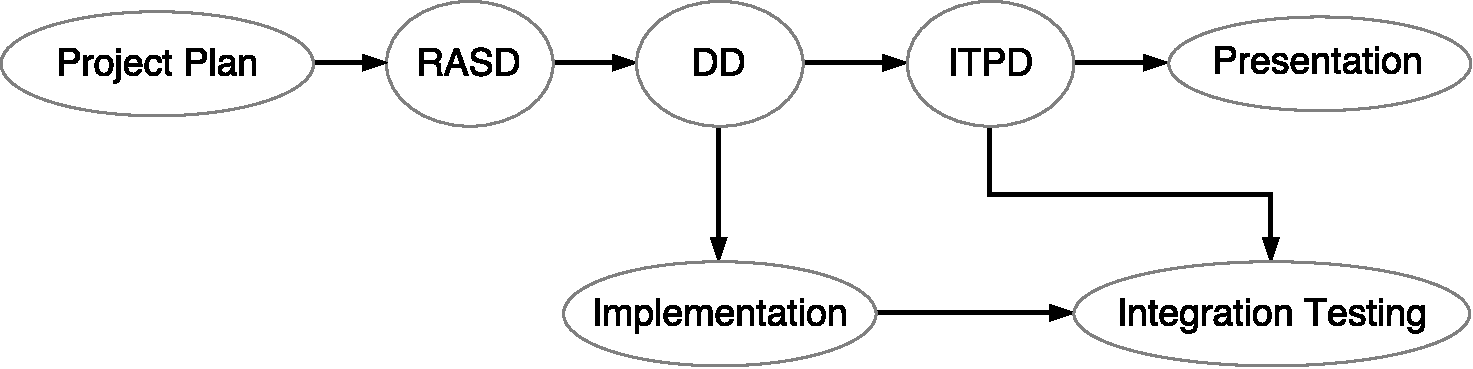
\includegraphics[width=\textwidth]{figures/TasksDAG.pdf}
    \caption{Directed Acyclic Graph showing the dependencies among tasks.}
    \label{fig:tasks-dag}
\end{figure}

\begin{table}[p]
    \centering
    \begin{tabular}{| l | l | l |}
        \hline
        \textbf{Activity}   & \textbf{Start Date}   & \textbf{Deadline} \\
        \hline
        RASD                & 2015-10-15            & 2015-11-06        \\
        DD                  & 2015-11-11            & 2015-12-04        \\
        ITPD                & 2016-01-07            & 2016-01-21        \\
        Project Plan        & 2016-01-21            & 2016-02-02        \\
        Presentation        & 2016-01-21            & 2016-02-09        \\
        Implementation      & 2016-?-?              & 2016-?-?          \\
        Integration Testing & 2016-?-?              & 2016-?-?          \\
        \hline
    \end{tabular}
    \caption{Schedule for project tasks.}
    \label{tab:schedule}
\end{table}

\begin{figure}[p]
    \hspace*{-1.5cm}
    \begin{ganttchart}[
        vgrid={*{6}{draw=none},dotted},
        time slot format=isodate,
        x unit=0.7mm,
        today=2016-02-02,
        today rule/.style= {blue, ultra thick},
        today label=Today,
        link bulge=6, link tolerance=5,
        bar inline label node/.style={font=\scriptsize},
        inline
        ]{2015-10-10}{2016-05-31}
        \gantttitlecalendar{year, month} \\
        \ganttbar[name=rasd]{RASD}{2015-10-15}{2015-11-06} \\
        \ganttbar[name=dd]{DD}{2015-11-11}{2015-12-04} \\
        \ganttbar[name=itpd]{ITPD}{2016-01-07}{2016-01-21} \\
        \ganttbar[name=pplan]{Plan}{2016-01-21}{2016-02-02} \\
        \ganttbar[name=pres]{Present.}{2016-01-21}{2016-02-09} \\
        \ganttbar[name=impl]{Implementation}{2016-02-15}{2016-05-01} \\
        \ganttbar[name=int-test]{Int. Testing}{2016-05-01}{2016-05-30}
        \ganttlink{rasd}{dd}
        \ganttlink{dd}{itpd}
        \ganttlink{impl}{int-test}
    \end{ganttchart}
    \hspace*{-1.5cm}
    \caption{Gantt chart of the project.}
    \label{fig:gantt}
\end{figure}
